%%**************************************************************
%% Vorlage fuer Bachelorarbeiten (o.ä.) der DHBW
%%
%% Autor: Tobias Dreher, Yves Fischer
%% Datum: 06.07.2011
%%
%% Autor: Michael Gruben
%% Datum: 15.05.2013
%%
%% Autor: Markus Barthel
%% Datum: 22.08.2014
%%**************************************************************

%!TEX root = ../dokumentation.tex

%
% Nahezu alle Einstellungen koennen hier getaetigt werden
%
	
\RequirePackage[l2tabu, orthodox]{nag}	% weist in Commandozeile bzw. log auf veraltete LaTeX Syntax hin

\documentclass[%
	pdftex,
	oneside,			% Einseitiger Druck.
	12pt,				% Schriftgroesse
	parskip=half,		% Halbe Zeile Abstand zwischen Absätzen.
%	topmargin = 10pt,	% Abstand Seitenrand (Std:1in) zu Kopfzeile [laut log: unused]
	headheight = 12pt,	% Höhe der Kopfzeile
%	headsep = 30pt,	% Abstand zwischen Kopfzeile und Text Body  [laut log: unused]
	headsepline,		% Linie nach Kopfzeile.
	footsepline,		% Linie vor Fusszeile.
	footheight = 16pt,	% Höhe der Fusszeile
	abstracton,		% Abstract Überschriften
	DIV=calc,		% Satzspiegel berechnen
	BCOR=8mm,		% Bindekorrektur links: 8mm
	headinclude=false,	% Kopfzeile nicht in den Satzspiegel einbeziehen
	footinclude=false,	% Fußzeile nicht in den Satzspiegel einbeziehen
	listof=totoc,		% Abbildungs-/ Tabellenverzeichnis im Inhaltsverzeichnis darstellen
	toc=bibliography,	% Literaturverzeichnis im Inhaltsverzeichnis darstellen
]{scrreprt}	% Koma-Script report-Klasse, fuer laengere Bachelorarbeiten alternativ auch: scrbook

% Einstellungen laden
\usepackage{xstring}
\usepackage[utf8]{inputenc}
\usepackage[T1]{fontenc}

\newcommand{\einstellung}[1]{%
  \expandafter\newcommand\csname #1\endcsname{}
  \expandafter\newcommand\csname setze#1\endcsname[1]{\expandafter\renewcommand\csname#1\endcsname{##1}}
}
\newcommand{\langstr}[1]{\einstellung{lang#1}}

\einstellung{matrikelnr}
\einstellung{titel}
\einstellung{kurs}
\einstellung{datumAbgabe}
\einstellung{firma}
\einstellung{firmenort}
\einstellung{abgabeort}
\einstellung{abschluss}
\einstellung{studiengang}
\einstellung{dhbw}
\einstellung{betreuer}
\einstellung{gutachter}
\einstellung{zeitraum}
\einstellung{arbeit}
\einstellung{autor}
\einstellung{sprache}
\einstellung{schriftart}
\einstellung{seitenrand}
\einstellung{kapitelabstand}
\einstellung{spaltenabstand}
\einstellung{zeilenabstand}
\einstellung{zitierstil}
 % verfügbare Einstellungen
%%%%%%%%%%%%%%%%%%%%%%%%%%%%%%%%%%%%%%%%%%%%%%%%%%%%%%%%%%%%%%%%%%%%%%%%%%%%%%%
%                                   Einstellungen
%
% Hier können alle relevanten Einstellungen für diese Arbeit gesetzt werden.
% Dazu gehören Angaben u.a. über den Autor sowie Formatierungen.
%
%
%%%%%%%%%%%%%%%%%%%%%%%%%%%%%%%%%%%%%%%%%%%%%%%%%%%%%%%%%%%%%%%%%%%%%%%%%%%%%%%


%%%%%%%%%%%%%%%%%%%%%%%%%%%%%%%%%%%% Sprache %%%%%%%%%%%%%%%%%%%%%%%%%%%%%%%%%%%
%% Aktuell sind Deutsch und Englisch unterstützt.
%% Es werden nicht nur alle vom Dokument erzeugten Texte in
%% der entsprechenden Sprache angezeigt, sondern auch weitere
%% Aspekte angepasst, wie z.B. die Anführungszeichen und
%% Datumsformate.
\setzesprache{de} % oder en
%%%%%%%%%%%%%%%%%%%%%%%%%%%%%%%%%%%%%%%%%%%%%%%%%%%%%%%%%%%%%%%%%%%%%%%%%%%%%%%%

%%%%%%%%%%%%%%%%%%%%%%%%%%%%%%%%%%% Angaben  %%%%%%%%%%%%%%%%%%%%%%%%%%%%%%%%%%%
%% Die meisten der folgenden Daten werden auf dem
%% Deckblatt angezeigt, einige auch im weiteren Verlauf
%% des Dokuments.
\setzematrikelnr{7474265}
\setzekurs{TINF-18B}
\setzetitel{Konzeption und Implementierung einer REST-basierten Schnittstelle zum Kopieren von Jira-Projekten}
\setzedatumAbgabe{Februar 2020}
\setzefirma{camos Software und Beratung GmbH}
\setzefirmenort{Stuttgart}
\setzeabgabeort{Stuttgart}
\setzestudiengang{Informatik}
\setzedhbw{Stuttgart}
\setzebetreuer{M.Sc. Markus Riegger}
\setzegutachter{UNBEKANNT}
\setzezeitraum{12 Wochen}
\setzearbeit{Praxisbericht 2 - T2000}
\setzeautor{Luca Stanger}
%%%%%%%%%%%%%%%%%%%%%%%%%%%%%%%%%%%%%%%%%%%%%%%%%%%%%%%%%%%%%%%%%%%%%%%%%%%%%%%%

%%%%%%%%%%%%%%%%%%%%%%%%%%%% Literaturverzeichnis %%%%%%%%%%%%%%%%%%%%%%%%%%%%%%
%% Bei Fehlern während der Verarbeitung bitte in ads/header.tex bei der
%% Einbindung des Pakets biblatex (ungefähr ab Zeile 110,
%% einmal für jede Sprache), biber in bibtex ändern.
\newcommand{\ladeliteratur}{%
\addbibresource{bibliographie.bib}
%\addbibresource{weitereDatei.bib}
}
%% Zitierstil
%% siehe: http://ctan.mirrorcatalogs.com/macros/latex/contrib/biblatex/doc/biblatex.pdf (3.3.1 Citation Styles)
%% mögliche Werte z.B numeric-comp, alphabetic, authoryear
%%\setzezitierstil{numeric-comp}
\setzezitierstil{alphabetic}
%%%%%%%%%%%%%%%%%%%%%%%%%%%%%%%%%%%%%%%%%%%%%%%%%%%%%%%%%%%%%%%%%%%%%%%%%%%%%%%%

%%%%%%%%%%%%%%%%%%%%%%%%%%%%%%%%% Layout %%%%%%%%%%%%%%%%%%%%%%%%%%%%%%%%%%%%%%%
%% Verschiedene Schriftarten
% laut nag Warnung: palatino obsolete, use mathpazo, helvet (option scaled=.95), courier instead
\setzeschriftart{lmodern} % palatino oder goudysans, lmodern, libertine

%% Paket um Textteile drehen zu können
%\usepackage{rotating}
%% Paket um Seite im Querformat anzuzeigen
%\usepackage{lscape}

%% Seitenränder
\setzeseitenrand{2.5cm}

%% Abstand vor Kapitelüberschriften zum oberen Seitenrand
\setzekapitelabstand{20pt}

%% Spaltenabstand
\setzespaltenabstand{10pt}
%%Zeilenabstand innerhalb einer Tabelle
\setzezeilenabstand{1.5}
%%%%%%%%%%%%%%%%%%%%%%%%%%%%%%%%%%%%%%%%%%%%%%%%%%%%%%%%%%%%%%%%%%%%%%%%%%%%%%%%

%%%%%%%%%%%%%%%%%%%%%%%%%%%%% Verschiedenes  %%%%%%%%%%%%%%%%%%%%%%%%%%%%%%%%%%%
%% Farben (Angabe in HTML-Notation mit großen Buchstaben)
\newcommand{\ladefarben}{%
	\definecolor{LinkColor}{HTML}{00007A}
	\definecolor{ListingBackground}{HTML}{FCF7DE}
}
%% Mathematikpakete benutzen (Pakete aktivieren)
%\usepackage{amsmath}
%\usepackage{amssymb}

%% Programmiersprachen Highlighting (Listings)
\newcommand{\listingsettings}{%
	\lstset{%
		language=Java,			% Standardsprache des Quellcodes
		numbers=left,			% Zeilennummern links
		stepnumber=1,			% Jede Zeile nummerieren.
		numbersep=5pt,			% 5pt Abstand zum Quellcode
		numberstyle=\tiny,		% Zeichengrösse 'tiny' für die Nummern.
		breaklines=true,		% Zeilen umbrechen wenn notwendig.
		breakautoindent=true,	% Nach dem Zeilenumbruch Zeile einrücken.
		postbreak=\space,		% Bei Leerzeichen umbrechen.
		tabsize=2,				% Tabulatorgrösse 2
		basicstyle=\ttfamily\footnotesize, % Nichtproportionale Schrift, klein für den Quellcode
		showspaces=false,		% Leerzeichen nicht anzeigen.
		showstringspaces=false,	% Leerzeichen auch in Strings ('') nicht anzeigen.
		extendedchars=true,		% Alle Zeichen vom Latin1 Zeichensatz anzeigen.
		captionpos=b,			% sets the caption-position to bottom
		backgroundcolor=\color{ListingBackground}, % Hintergrundfarbe des Quellcodes setzen.
		xleftmargin=0pt,		% Rand links
		xrightmargin=0pt,		% Rand rechts
		frame=single,			% Rahmen an
		frameround=ffff,
		rulecolor=\color{darkgray},	% Rahmenfarbe
		fillcolor=\color{ListingBackground},
		keywordstyle=\color[rgb]{0.133,0.133,0.6},
		commentstyle=\color[rgb]{0.133,0.545,0.133},
		stringstyle=\color[rgb]{0.627,0.126,0.941}
	}
}

%%%%%%%%%%%%%%%%%%%%%%%%%%%%%%%%%%%%%%%%%%%%%%%%%%%%%%%%%%%%%%%%%%%%%%%%%%%%%%%%

%%%%%%%%%%%%%%%%%%%%%%%%%%%%%%%% Eigenes %%%%%%%%%%%%%%%%%%%%%%%%%%%%%%%%%%%%%%%
%% Hier können Ergänzungen zur Präambel vorgenommen werden (eigene Pakete, Einstellungen)

\usepackage{pdflscape}
\usepackage{longtable}
\usepackage{xcolor,colortbl}

%% Created by LUS. 29.01.2020
%% Prettyref Formate
\newcommand*{\itmref}[1]{FA-\ref{#1}}

%% Created by LUS. 10.12.2019
%% Prettyref Formate
\usepackage{prettyref}
\newrefformat{sec}{Abschnitt \ref{#1} auf Seite \pageref{#1}}

%% Created by LUS. 07.01.2020
%% Fullref Formate
\newcommand*{\fullref}[1]{Anhang \nameref{#1}}

%% Created by LUS. 08.01.2020
%% Compref Formate
\newcommand*{\compref}[1]{\nameref*{#1} (vgl. \hyperref[{#1}]{\autoref*{#1}})} % lese Einstellungen

\newcommand{\iflang}[2]{%
  \IfStrEq{\sprache}{#1}{#2}{}
}

\langstr{abkverz}
\langstr{anhang}
\langstr{glossar}
\langstr{deckblattabschlusshinleitung}
\langstr{artikelstudiengang}
\langstr{studiengang}
\langstr{anderdh}
\langstr{von}
\langstr{dbbearbeitungszeit}
\langstr{dbmatriknr}
\langstr{dbkurs}
\langstr{dbfirma}
\langstr{dbbetreuer}
\langstr{dbgutachter}
\langstr{sperrvermerk}
\langstr{erklaerung}
\langstr{abstract}
\langstr{listingname}
\langstr{listlistingname}
\langstr{listingautorefname}
 % verfügbare Strings
\input{lang/\sprache} % Übersetzung einlesen

% Einstellung der Sprache des Paketes Babel und der Verzeichnisüberschriften
\iflang{de}{\usepackage[english, ngerman]{babel}}
\iflang{en}{\usepackage[ngerman, english]{babel}} 


%%%%%%% Package Includes %%%%%%%

\usepackage[margin=\seitenrand,foot=1cm]{geometry}	% Seitenränder und Abstände
\usepackage[activate]{microtype} %Zeilenumbruch und mehr
\usepackage[onehalfspacing]{setspace}
\usepackage{makeidx}
\usepackage[autostyle=true,german=quotes]{csquotes}
\usepackage{longtable}
\usepackage{enumitem}	% mehr Optionen bei Aufzählungen
\usepackage{graphicx}
\usepackage{pdfpages}   % zum Einbinden von PDFs
\usepackage{xcolor} 	% für HTML-Notation
\usepackage{float}
\usepackage{array}
\usepackage{calc}		% zum Rechnen (Bildtabelle in Deckblatt)
\usepackage[right]{eurosym}
\usepackage{wrapfig}
\usepackage{pgffor} % für automatische Kapiteldateieinbindung
\usepackage[perpage, hang, multiple, stable]{footmisc} % Fussnoten
\usepackage[printonlyused]{acronym} % falls gewünscht kann die Option footnote eingefügt werden, dann wird die Erklärung nicht inline sondern in einer Fußnote dargestellt
\usepackage{listings}

% Notizen. Einsatz mit \todo{Notiz} oder \todo[inline]{Notiz}. 
\usepackage[obeyFinal,backgroundcolor=yellow,linecolor=black]{todonotes}
% Alle Notizen ausblenden mit der Option "final" in \documentclass[...] oder durch das auskommentieren folgender Zeile
% \usepackage[disable]{todonotes}

% Kommentarumgebung. Einsatz mit \comment{}. Alle Kommentare ausblenden mit dem Auskommentieren der folgenden und dem aktivieren der nächsten Zeile.
\newcommand{\comment}[1]{\par {\bfseries \color{blue} #1 \par}} %Kommentar anzeigen
% \newcommand{\comment}[1]{} %Kommentar ausblenden


%%%%%% Configuration %%%%%

%% Anwenden der Einstellungen

\usepackage{\schriftart}
\ladefarben{}

% Titel, Autor und Datum
\title{\titel}
\author{\autor}
\date{\datum}

% PDF Einstellungen
\usepackage[%
	pdftitle={\titel},
	pdfauthor={\autor},
	pdfsubject={\arbeit},
	pdfcreator={pdflatex, LaTeX with KOMA-Script},
	pdfpagemode=UseOutlines, 		% Beim Oeffnen Inhaltsverzeichnis anzeigen
	pdfdisplaydoctitle=true, 		% Dokumenttitel statt Dateiname anzeigen.
	pdflang={\sprache}, 			% Sprache des Dokuments.
]{hyperref}

% (Farb-)einstellungen für die Links im PDF
\hypersetup{%
	colorlinks=true, 		% Aktivieren von farbigen Links im Dokument
	linkcolor=LinkColor, 	% Farbe festlegen
	citecolor=LinkColor,
	filecolor=LinkColor,
	menucolor=LinkColor,
	urlcolor=LinkColor,
	linktocpage=true, 		% Nicht der Text sondern die Seitenzahlen in Verzeichnissen klickbar
	bookmarksnumbered=true 	% Überschriftsnummerierung im PDF Inhalt anzeigen.
}
% Workaround um Fehler in Hyperref, muss hier stehen bleiben
\usepackage{bookmark} %nur ein latex-Durchlauf für die Aktualisierung von Verzeichnissen nötig

% Schriftart in Captions etwas kleiner
\addtokomafont{caption}{\small}

% Literaturverweise (sowohl deutsch als auch englisch)
\iflang{de}{%
\usepackage[
	backend=biber,		% biber empfohlen. Falls biber Probleme macht: bibtex
	bibwarn=true,
	bibencoding=utf8,	% wenn .bib in utf8, sonst ascii
	sortlocale=de_DE,
	maxcitenames=1,
	style=\zitierstil,
]{biblatex}
%%\DeclareLanguageMapping{ngerman}{ngerman-apa}
\DefineBibliographyStrings{ngerman}{
   andothers = {{et\,al\adddot}},
}
}
\iflang{en}{%
\usepackage[
	backend=biber,		% empfohlen. Falls biber Probleme macht: bibtex
	bibwarn=true,
	bibencoding=utf8,	% wenn .bib in utf8, sonst ascii
	sortlocale=en_US,
	style=\zitierstil,
]{biblatex}
}

\ladeliteratur{}

% Glossar
\usepackage[nonumberlist,toc]{glossaries}

%%%%%% Additional settings %%%%%%

% Hurenkinder und Schusterjungen verhindern
% http://projekte.dante.de/DanteFAQ/Silbentrennung
\clubpenalty = 10000 % schließt Schusterjungen aus (Seitenumbruch nach der ersten Zeile eines neuen Absatzes)
\widowpenalty = 10000 % schließt Hurenkinder aus (die letzte Zeile eines Absatzes steht auf einer neuen Seite)
\displaywidowpenalty=10000

% Bildpfad
\graphicspath{{images/}}

% Einige häufig verwendete Sprachen
\lstloadlanguages{PHP,Python,Java,C,C++,bash}
\listingsettings{}
% Umbennung des Listings
\renewcommand\lstlistingname{\langlistingname}
\renewcommand\lstlistlistingname{\langlistlistingname}
\def\lstlistingautorefname{\langlistingautorefname}

% Abstände in Tabellen
\setlength{\tabcolsep}{\spaltenabstand}
\renewcommand{\arraystretch}{\zeilenabstand}


\makeglossaries
%!TEX root = ../dokumentation.tex

%
% vorher in Konsole folgendes aufrufen:
%	makeglossaries makeglossaries dokumentation.acn && makeglossaries dokumentation.glo
%

%
% Glossareintraege --> referenz, name, beschreibung
% Aufruf mit \gls{...}
%
\newglossaryentry{Glossareintrag}{name={Glossareintrag},plural={Glossareinträge},description={Ein Glossar beschreibt verschiedenste Dinge in kurzen Worten}}


\begin{document}

	% Deckblatt
	\begin{spacing}{1}
		%!TEX root = ../dokumentation.tex

\begin{titlepage}
	\begin{longtable}{p{8.2cm} p{5.4cm}}
		%{\raisebox{\ht\strutbox-\totalheight}{\includegraphics{images/camos_Logo}}} &
		{\raisebox{\ht\strutbox-\totalheight}{
\includegraphics[height=2.5cm]{images/dhbw.png}}}
	\end{longtable}
	\enlargethispage{20mm}
	\begin{center}
		\vspace*{12mm}	{\LARGE\textbf \titel }\\
		\vspace*{12mm}	{\large\textbf \arbeit}\\
		\vspace*{12mm}	\langartikelstudiengang{} \langstudiengang{} \studiengang\\
    \vspace*{3mm}		\langanderdh{} \dhbw\\
		\vspace*{12mm}	\langvon\\
		\vspace*{3mm}		{\large\textbf \autor}\\
		\vspace*{12mm}	\datumAbgabe\\
	\end{center}
	\vfill
	\begin{spacing}{1.2}
	\begin{tabbing}
		mmmmmmmmmmmmmmmmmmmmmmmmmm             \= \kill
		\textbf{\langdbbearbeitungszeit}       \>  \zeitraum\\
		\textbf{\langdbmatriknr, \langdbkurs}  \>  \matrikelnr, \kurs\\
		\textbf{\langdbfirma}                  \>  \firma, \firmenort\\
		\textbf{\langdbgutachter}               \>  \gutachter\\
	\end{tabbing}
	\end{spacing}
\end{titlepage}

	\end{spacing}
	\newpage

	\pagenumbering{Roman}

	\pagestyle{plain}		% nur Seitenzahlen im Fuß
	
	\RedeclareSectionCommand[beforeskip=\kapitelabstand         ]{chapter} % stellt Abstand vor Kapitelüberschriften ein

	% Inhaltsverzeichnis
	\begin{spacing}{1.1}
		\begingroup
		
			% auskommentieren für Seitenzahlen unter Inhaltsverzeichnis
			\renewcommand*{\chapterpagestyle}{empty}
			\pagestyle{empty}
			
			
			\setcounter{tocdepth}{2}
			%für die Anzeige von Unterkapiteln im Inhaltsverzeichnis
			%\setcounter{tocdepth}{2}
			
			\tableofcontents
			\clearpage
		\endgroup
	\end{spacing}
	\newpage

	% Abbildungsverzeichnis
	\cleardoublepage
	\listoffigures

	%Tabellenverzeichnis
	\cleardoublepage
	\listoftables
	\cleardoublepage

	\pagenumbering{arabic}
	
	\pagestyle{headings}		% Kolumnentitel im Kopf, Seitenzahlen im Fuß


	%!TEX root = ../dokumentation.tex

\chapter{Chapter1}
Chapter1


	
	%!TEX root = ../dokumentation.tex
\chapter{Entwicklung}
Für die Entwicklung der Software wurde von Florian die IDE Visual Studio Code verwendet und von Luca die IDE Jetbrains PhpStorm.
Zum Verwalten der Datenbank wurde die Software Jetbrains DataGrip.

\section{Toolchain}

\section{Bibliotheken/Frameworks}
\subsection{Bower}
\subsection{Composer}
\subsection{phpunit}

\section{MVC}
\subsection{.htaccess}
\subsection{Model}
\subsection{View}
\subsection{Controller}

\section{Funktionalität}

\subsection{Login/Register}
passwort hashing
confirm ohne email wegen email server in aws.
logik der registrierung und anmeldung

\subsection{Lobby}

\subsubsection{Scrum Master}
\subsubsection{Spieler}
	
	%!TEX root = ../dokumentation.tex
\chapter{Hosting}\label{ch:hosting}

\section{Anbieter}
Zuerst wurde der Anbieter \href{https://azure.microsoft.com/de-de/}{Microsoft Azure} zum Hosten der Datenbank und des PHP Servers vorgezogen. Als Student erhält man, über das \href{https://education.github.com/pack}{Github Student Developer Pack}, ein jährliches Budget von 100\$ ohne Angabe einer Kreditkarte bzw. Bezahlmethode. Azure wurde bereits bei einem Projekt aus dem dritten Semester als Anbieter verwendet. Jedoch mit dem Studentenabonnement konnten aus unbekannten Gründen keine Server und Datenbanken in Europa erstellt werden.\\
Aus Neugier und Interesse wurde danach der Anbieter \href{https://aws.amazon.com/de/}{Amazon Web Services (AWS)} verwendet. Ebenso erhält man, über das Github Student Developer Pack, ein Budget von 100\$ (damals 150\$).\\
Alle in diesem Projekt verwendeten Services sind in dem 12 monatigem \href{https://aws.amazon.com/de/free/}{kostenlosem Kontigent von AWS} inbegriffen.

\section{PHP Server}
Der PHP Server wird mit \href{https://aws.amazon.com/de/elasticbeanstalk/}{AWS Elastic Beanstalk} gehostet. \glqq AWS Elastic Beanstalk ist ein benutzerfreundlicher Service zum Bereitstellen und Skalieren von Webanwendungen und -Services\grqq. Anwendungen können mit Java, .NET, Node.js, Python, Ruby, Go, Docker und auch PHP bereitgestellt werden. Der Quellcode der Anwendung wird hochgeladen und Elastic Beanstalk übernimmt die automatische Bereitstellung. \cite{AWSEB}\\
Die Planning Poker Anwendung wird auf einem AWS Elastik Beanstalk 64bit Amazon Linux/2.9.4 Server mit der PHP Version 7.3 gehostet.

Damit der Elastic Beanstalk Server alle richtigen Konfigurationen durchführen kann, können \href{https://docs.aws.amazon.com/de_de/elasticbeanstalk/latest/dg/ebextensions.html}{Konfigurationsdateien} zum Quellcode hinzugefügt werden. Diese findet man in dem \href{https://github.com/Drinkler/Planning-Poker/tree/master/.ebextensions}{\lstinline{.ebextensions} Ordner}. In diesem Ordner befinden sich \lstinline{.config} Dateien. Durch die \lstinline{project.config} Datei werden alle benötigten Komponenten auf dem Server installiert.

	
	%!TEX root = ../dokumentation.tex
\chapter{Datenbank}

\section{Hosting}
Zum Hosten der Datenbank wird die \href{https://aws.amazon.com/de/rds/mariadb/}{Amazon RDS for MariaDB} mit der MariaDB Version 10.2.21 verwendet. \\
\glqq\href{https://aws.amazon.com/de/rds/}{Amazon Relational Database Service (Amazon RDS)} ist ein Webservice, der das Einrichten, Betreiben und Skalieren einer relationalen Datenbank in der AWS Cloud vereinfacht.\grqq  Amazon RDS unterstützt bis zu sechs verschiedene Datenbank-Engines, z.B. MySQL, PostgreSQL oder auch MariaDB. \cite{AWSRDS}

Der Vorteil einer Cloud-basierten Datenbank ist, dass jeder Entwickler problemlos darauf zugreifen kann.\\
Um auf diese Datenbank zugreifen zu können, unterstützt AWS sogenannte Security Groups. Diese Gruppen dienen als virtuelle Firewall. Man teilt sie einer Ressource wie z.B. der Datenbank oder dem Elastic Beanstalk Server zu. In einer Security Group wird spezifiziert, welche IPs und sonstigen Ressourcen Zugriff haben.\\
Da während der Entwicklungszeit die IP Adresse eines Entwicklers sich täglich geändert hat, wurde Zugriff von Überall erlaubt. Dies stellt natürlich ein erhöhtes Sicherheitsrisiko dar, dennoch braucht man Anmeldedaten für die Datenbank. Nach der Entwicklungsphase wurde dieser Zugang entfernt.

\section{Verwendung von \$\_SERVER}
Damit die Anmeldedaten für die Datenbank nicht blank im Quellcode zu finden sind, wurden diese in dem \$\_SERVER Array des Webservers gespeichert. Dieses Verfahren wurde gewählt, da ein öffentliches Github Repository erstellt wurde und somit sonst für jeden sichtbar wäre.

Um die Daten auf dem lokalen Xampp Server verwenden zu können, werden diese in der \lstinline{httpd-xampp.conf} gespeichert. Im folgenden Codeblock werden die Anmeldedaten im Modul \lstinline{env_module} definiert.
\newpage
\begin{lstlisting}[caption={httpd-xampp.conf Umgebungsvariablen}, language=bash]
#
# XAMPP settings
#

<IfModule env_module>
    ...
    SetEnv RDS_DB_NAME "planning_poker"
    SetEnv RDS_HOSTNAME "planning-poker.cztpemauxamy.eu-central-1.rds.amazonaws.com"
    SetEnv RDS_PASSWORD "<password>"
    SetEnv RDS_PORT "3306"
    SetEnv RDS_USERNAME "admin"
</IfModule>
\end{lstlisting}

Nun kann man innerhalb des Programmcodes auf das \$\_SERVER Array zugreifen um die zuvor definierten Werte aufzurufen. Dieser Codeblock, aus der Datei Model/ModelBase.php, zeigt die Funktion zur Erstellung der Datenbankverbindung. 

\begin{lstlisting}[caption={Funktion getPdo()}, language=PHP]
/**
* GetPDO: returns a PDO Connection
* @author Luca Stanger
* @return Database
*/
public function getPdo()
{
	if (self::$_db === null) {
		self::$_db = new \PlanningPoker\Model\Database(
			$_SERVER['RDS_HOSTNAME'],
			$_SERVER['RDS_PORT'],
			$_SERVER['RDS_DB_NAME'],
			$_SERVER['RDS_USERNAME'],
			$_SERVER['RDS_PASSWORD'],
			'utf8'
		);
	}

	return self::$_db;
}
\end{lstlisting}

Damit der AWS Elastic Beanstalk Server ebenfalls auf die Daten über \$\_SERVER zugreifen kann, werden diese unter den Konfigurationseinstellung in AWS als Umgebungseigenschaften definiert.

\section{Schema}
In der Abbildung \ref{datenbank} ist das Schema der Datenbank zu sehen.

\begin{figure}[H]
	\centering
  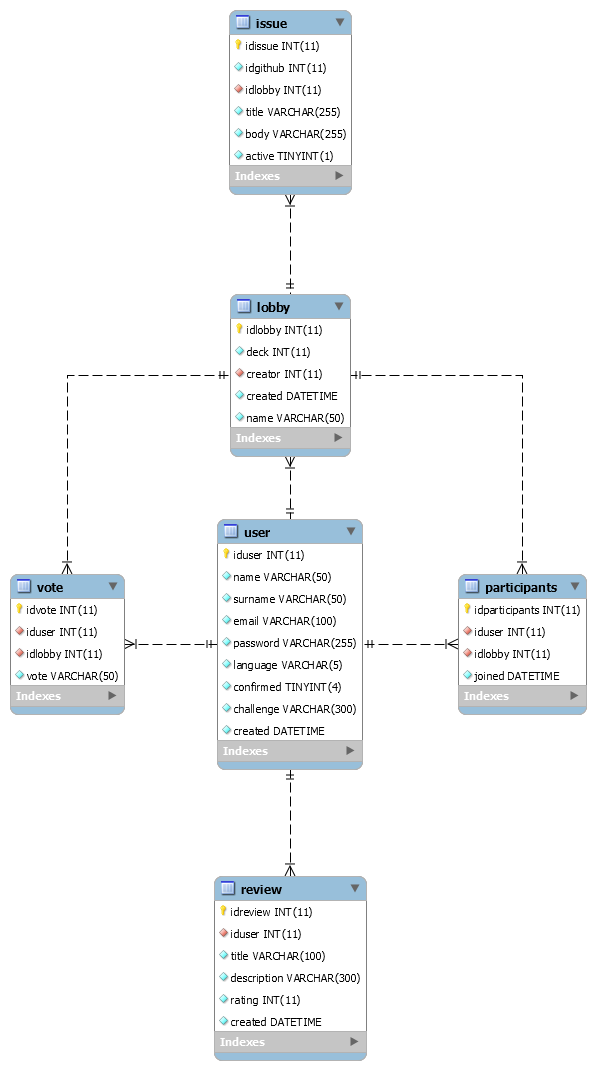
\includegraphics[width=0.74\textwidth]{images/database.png}
	\caption{Visualisierung der Datenbank}
	\label{datenbank}
\end{figure}

Zu sehen sind die einzelnen Tabellen der Datenbank mit Verknüpfungen zu anderen Tabellen. In einer Tabelle sind die einzelnen Spalten beschrieben. Primärschlüssel haben einen goldenen Schlüssel, Fremdschlüssel eine rote Raute und normale Spalten eine blaue Raute. Außerdem werden die Typen der Spalten gezeigt. Alle Verbindungen in diesem Schema beschreiben eine 1:N Beziehung mit ON DELETE CASCADE.

Der Vorteil dieses Schemas ist, dass keine überflüssigen Daten vorhanden bleiben. Wenn z.B. ein Benutzer sich löscht, werden automatisch alle Daten dieses Benutzers aus den verbundenen Tabellen gelöscht. Die Reviews, Votes, Participations und erstellten Lobbies des Benutzers werden gelöscht. Dadurch, dass eine Lobby gelöscht wird, werden die Issues dieser Lobby, die Votes und Participations gelöscht.
	
	%!TEX root = ../dokumentation.tex
\chapter{Continuous Integration}\label{ch:continuous-integration}
Am Anfang des Projektes wurde \href{https://aws.amazon.com/de/codepipeline/}{AWS CodePipeline} als Continuous Integration (CI) verwendet. Dies stellte eine einfache Lösung dar, da unter anderem Github als Drittanbieter verfügbar ist. Somit wurde bei jeder Code-Änderung auf dem Master Branch des Github Repositories das neue Projekt auf den Server geladen.\\
Jedoch als später Tests mit PHPUnit hinzugefügt wurden, wurde vorausgesetzt, dass vor jedem Build das Projekt getestet wird.\\
Dazu wäre \href{https://aws.amazon.com/de/codebuild/}{AWS CodeBuild} eine Möglichkeit gewesen. Doch, da bereits persönlich mit dem kostenlosem CI Tool \href{https://travis-ci.com/}{Travis CI} gearbeitet wurde, fiel die Wahl auf dieses.

Für die Verwendung von Travis CI benötigt es die Berechtigung auf das Github Repository zuzugreifen. Außerdem muss eine \href{https://github.com/Drinkler/Planning-Poker/blob/master/.travis.yml}{\lstinline{.travis.yml}} Datei im Root des Repositories liegen. In dieser yml-Datei werden die \href{https://docs.travis-ci.com/user/job-lifecycle/}{nacheinander ablaufenden Befehle} definiert. In diesen Schritten wird das Projekt gebaut und getestet. Schlägt der Build fehl, wird er abgebrochen und der Code wird nicht auf den Server geladen. Durch die Möglichkeit mit \href{https://docs.travis-ci.com/user/deployment/codedeploy/}{AWS CodeDeploy} wird das Projekt automatisch, nach einem erfolgreichem Build, hochgeladen.\\
Travis CI klont das Repository in eine neue virtuelle Umgebung und führt diesen Build aus. Der letzte Build des Projektes ist \href{https://travis-ci.com/github/Drinkler/Planning-Poker}{hier} zu finden.\\
Um keine Anmeldedaten des Deploy Schrittes im Quellcode stehen zu haben, wurden die \href{https://docs.travis-ci.com/user/environment-variables/}{Travis CI Umgebungsvariablen} verw endet.

Die Abbildung \ref{ci} zeigt den Ablauf zwischen den einzelnen Schritten von der Entwicklung bis zur Veröffentlichung. Ein lokales Git repräsentiert einen Entwickler. Dies ist für andere Projekte variierbar.

\begin{figure}[H]
	\centering
  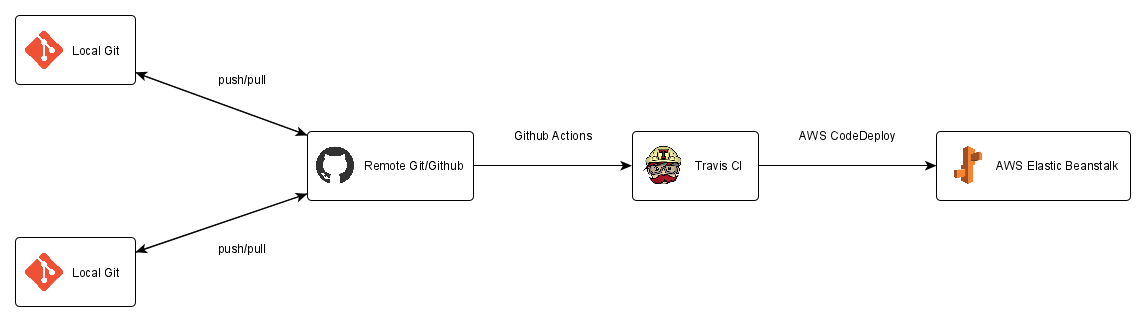
\includegraphics[width=\textwidth]{images/continuous_integration.png}
	\caption{Continuous Integration Prozess}
	\label{ci}
\end{figure}
	
	%!TEX root = ../dokumentation.tex
\chapter{Continuous Integration}\label{ch:continuous-integration}
Am Anfang des Projektes wurde \href{https://aws.amazon.com/de/codepipeline/}{AWS CodePipeline} als Continuous Integration (CI) verwendet. Dies stellte eine einfache Lösung dar, da unter anderem Github als Drittanbieter verfügbar ist. Somit wurde bei jeder Code-Änderung auf dem Master Branch des Github Repositories das neue Projekt auf den Server geladen.\\
Jedoch als später Tests mit PHPUnit hinzugefügt wurden, wollte man das vor jedem Build das Projekt getestet wird.\\
Dazu wäre \href{https://aws.amazon.com/de/codebuild/}{AWS CodeBuild} eine Möglichkeit gewesen. Doch, da bereits persönlich mit dem kostenlosem CI Tool \href{https://travis-ci.com/}{Travis CI} gearbeitet wurde, wurde dies ausgewählt.

Für die Verwendung von Travis CI benötigt es die Berechtigung auf das Github Repository zuzugreifen. Außerdem muss eine \href{https://github.com/Drinkler/Planning-Poker/blob/master/.travis.yml}{\lstinline{.travis.yml}} Datei im Root des Repositories liegen. In dieser yml-Datei werden die \href{https://docs.travis-ci.com/user/job-lifecycle/}{nacheinander ablaufenden Befehle} definiert. In diesen Schritten wird das Projekt gebaut und getestet. Schlägt der Build fehl, wird er abgebrochen und der Code wird nicht auf den Server geladen. Durch die Möglichkeit mit \href{https://docs.travis-ci.com/user/deployment/codedeploy/}{AWS CodeDeploy} wird das Projekt automatisch, nach einem erfolgreichem Build, hochgeladen.\\
Travis CI klont das Repository in eine neue virtuelle Umgebung und führt diesen Build aus. Der letzte Build des Projektes ist \href{https://travis-ci.com/github/Drinkler/Planning-Poker}{hier} zu finden.\\
Um keine Anmeldedaten des Deploy Schrittes im Quellcode stehen zu haben, wurden die \href{https://docs.travis-ci.com/user/environment-variables/}{Travis CI Umgebungsvariablen} verwendet.

Die Abbildung \ref{ci} zeigt den Ablauf zwischen den einzelnen Schritten von der Entwicklung bis zur Veröffentlichung. Ein lokales Git repräsentiert einen Entwickler. Dies ist für andere Projekte variierbar.

\begin{figure}[H]
	\centering
  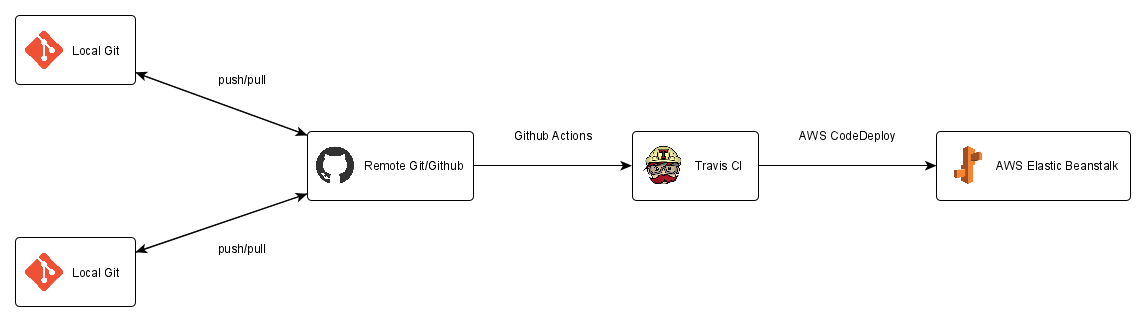
\includegraphics[width=\textwidth]{images/continuous_integration.png}
	\caption{Continuous Integration Prozess}
	\label{ci}
\end{figure}
	
	\clearpage

	% Literaturverzeichnis
	\cleardoublepage
	\printbibliography

	% Glossar
	\printglossary[style=altlist,title=\langglossar]
	
\end{document}
≥